\documentclass[9pt]{article}

\usepackage{graphicx} % Required for inserting images
\usepackage{amsmath}
\usepackage{amssymb}
\usepackage{amsfonts}
\usepackage{ctex}
\usepackage{enumitem}
\usepackage{longtable}
\usepackage{makecell} % 换行

% 使用分栏宏包
\usepackage{multicol}
\usepackage{multirow}
\setlength{\columnseprule}{0.4pt} % 分割线

% 设置字体
\usepackage{unicode-math}
\setmainfont{Cambria}
\setmathfont{Cambria Math}

% 调整页面布局
\usepackage[a4paper, top=0.7cm, bottom=1cm, left=0.7cm, right=.7cm]{geometry}
\setlength{\footskip}{15pt}

% 设置页脚/页眉
\usepackage{fancyhdr}
\fancyfoot[C]{{\scriptsize $\xi_i,\eta_i$ 默认是向量 | } $\mathbf{v}_{\intercal}$ {\scriptsize 代表转置，如果后面也是就不再重复写} | Copyright By Jingren Zhou | Page \thepage}
\fancyhead[]{}
\pagestyle{fancy}
% 去除线
\renewcommand{\headrulewidth}{0pt}
\renewcommand{\footrulewidth}{0pt}

% 设置 section/subsection 之间的行间距
\usepackage{titlesec}
\titlespacing*{\section}{0pt}{0pt}{0pt}
\titlespacing*{\subsection}{0pt}{0pt}{0pt}

% 调整标题上下间距
\usepackage{titling}
\setlength{\droptitle}{-2.4cm} % 负值表示向上移动

% 设置标题，作者，时间
\title{HDE Note}
\author{}
\date{}

% 正文
\begin{document}


% 标题
\maketitle
\thispagestyle{fancy}
\vspace{-3.5cm}

% 字体大小
\fontsize{10pt}{11pt}\selectfont
\setlength{\parindent}{0pt}


\section{Basic Knowledge} % Basic Knowledge

\subsection{Linear Algebra}

\textbf{Operations of Matrix Determinant}: $det(kA)=k^ndet(A)$ ; \ $det(A^{-1})=det(A)^{-1}$ ; \ $(AB)^*=B^*A^*$ ; \ $det(A)=det(A^T)$.

\textbf{Eigenvalue $\lambda$ and Eigenvector $\mathbf{x}$}: $A\mathbf{x}=\lambda\mathbf{x}$. \ \ 1.Using $det(A-\lambda I)=0$ to found $\lambda$. \ \ 2.Using $(A-\lambda I)\mathbf{x}=0$ to found $\mathbf{x}$.

$\cdot$ \textbf{Algebraic Multiplicity} of an eigenvalue: $\lambda$ 重复出现的次数. \ \ \ $\geq$ \ \ \ $\cdot$ \textbf{Geometric Multiplicity} of an eigenvalue: \# $\mathbf{x}$ under $\lambda$.

\textbf{Generalised Eigenvectors}: If $\lambda$ (AM>GM): Using $\xi_\lambda = (A-\lambda\mathbb{I})\eta_1,\eta_{n-1} = (A-\lambda\mathbb{I})\eta_{n}$ for each $\xi_\lambda$ to find all \textit{generalised eigenvectors}.


\subsection{ODE / PDE Definitions}

\textbf{Def of DEs / ODEs / PDEs}: Given independent variables ( $x_1,...,x_n$ ), functions ( $y_1(x_{j_1}),...,y_p(x_{j_p})$ ) and some derivatives (e.g. $\partial_s y_t$).

$\cdot$ \textbf{DEs} if: $\mathcal{F}_i[y_r,...,\partial_{x_t}y_b,x_1,...,x_n]=0,\ \ \  i=s,s-1,...,1.$ \ \ \ $\cdot$ \textbf{ODEs}: $n=1$ {\small (无偏导)} \ \ $\cdot$ \textbf{PDEs}: $n>1$ {\small (有偏导)}

\textbf{Def of Linear / Order}: Let $L$ be the terms by collecting all the $y_i(x_s)$ (dependent) terms. (e.g. $L=\frac{d^2}{dx^2}-x$ for $y''(x)-xy(x)=x^2$)

$\cdot$ DE is \textbf{Linear} if: $L[a_1y_1+a_2y_2]=a_1L[y_1]+a_2L[y_2]$ \ \ \ \ ( OR: {\small 所有$y_i^{(n)}$是线性的} ) \ \ \ $\cdot$ \textbf{n-th order ODEs}: $\mathbf{y}^{(n)}(x)=\mathbf{F}(\mathbf{y}_{\intercal },\mathbf{y}',...,\mathbf{y}^{(n-1)},x)$


\subsection{Calculus \& Single ODE / PDE Solution Method}

\textbf{Gradient $\nabla$}: $\nabla F=(\partial_xF,\partial_yF,\partial_zF,...)$ \ \ \ \ \ \ \textbf{(non-)Simply Connected}: {\footnotesize (没)有洞,相互连接的区域} \ \ \ \ \ \ \textbf{$\partial D$}: D区域的边界

\textbf{Seperable 1st ODE form}: $\frac{dy}{dx}=\frac{f(x)}{g(y)}$. $\Rightarrow$ 直接解就行. \ \ \ \ \textbf{Linear 1st ODE form}: $y'+p(x)y=q(x)$. $\Rightarrow$ $e^{\int p(x)dx}y=\int q(x)\cdot e^{\int p(x)dx}dx$

\textbf{Homogeneous 2nd ODE with constant coefficients}: $ay''+by'+c=0$ $\Rightarrow$ Calculate $ar^2+br+c=0$ and $\Delta=b^2-4ac$.

1. $\Delta>0$,$y=C_1e^{r_1x}+C_2e^{r_2x}$; \ \ 2. $\Delta=0$,$y=(C_1+C_2x)e^{rx}$; \ \ 3. $\Delta<0$,$y=e^{\alpha x}(C_1cos(\beta x)+C_2sin(\beta x))$ ps: $r_1,r_2 = \alpha\pm\beta i$

% \textbf{non-Homogeneous 2nd ODE with constant coefficients}: $ay''+by'+c=g(x)$ $\Rightarrow$ Solution = $y_c+y_p$ \ \ \ ps:$y_c$ is sol for $g(x)=0$.

% $\cdot$ Method of Undetermined Coefficients: Let $A_n(x)=\sum_{i=0}^{n}a_ix^i, \ \ B_n(x)=\sum_{i=0}^{n}b_ix^i, \ \ P_n(x)=\sum_{i=0}^{n}p_ix^i$.

% \begin{enumerate}[itemsep=-2pt, topsep=-2pt]
%    \item If $g(x)=P_n(x)$ \ $\Rightarrow$ \ $y_p=x^sA_n(x)$ \ , $s:= \ \ 0,(0\ne r_1,r_2); \ \ 1,(0 = r_1 \ or \ r_2); \ \ 2,(0 = r_1 = r_2).$
%    \item If $g(x)=Me^{kx}$ \ $\Rightarrow$ \ $y_p=Cx^se^{kx}$ \ , $s:= \ \ 0,(k\ne r_1,r_2); \ \ 1,(k = r_1 \ or \ r_2); \ \ 2,(k = r_1 = r_2).$
%    \item If $g(x)=Mcos(kx)+Nsin(kx)$ \ $\Rightarrow$ \ $y_p=x^s(C_1cos(kx)+C_2sin(kx))$ \ , $s:= \ \ 0,(r_1,r_2 \ne ik); \ \ 1,(r_1,r_2= ik).$
%    \item If $g(x)=$ product from 1,2,3. \ $\Rightarrow$ \ $y_p=$ corresponding product of $y_p$ ($x^s$ 只乘一次) \ , \ $s:=$ 令$y_p$与$y_c$没有相同项. ($\leq 2$)
% \end{enumerate}

% $\cdot$ Method of Variation of Parameters: Suppose $y_c(x)=C_1y_1(x)+C_2y_2(x)$. \ \ $W(y_1,y_2)=det$ {\scriptsize $\begin{pmatrix}y_1 & y_2 \\ y'_1 & y'_2 \end{pmatrix}$} (Wronskian)

% \ \ \ \ \ \ Then $y_p=-y_1(x)\int\frac{y_2(x)g(x)}{aW(y_1,y_2)}dx + y_2(x)\int\frac{y_1(x)g(x)}{aW(y_1,y_2)}dx$.


\section{Systems of First-Order Linear Equations (ODEs)} % Systems of First-Order Linear Equations

\subsection{Introduce to First-Order ODEs}

\vspace{-0.25cm}
{\tiny * 此节只考虑 First-Order ,所有定理描述都是 First-Order version}
\vspace{-0.15cm}

\textbf{n-th ODE $\rightarrow$ 1st ODE}: For $y^{(n)}=F(y,y',...,y^{(n-1)},x)$, Let $x_i=y^{(i-1)}$. Then $x'_n=F(x_1,x_2,...,x_{n-1})$ which is 1st ODE.

\textbf{Existence \& Uniqueness Theorem}: Given $\mathbf{y}'(x)=\mathbf{f}(x,\mathbf{y}_{\intercal}),\mathbf{y}(x_0)=\mathbf{y_0}$. Let $R_i=[x_0-t,x_0+t]\times\prod_i[y_{0_i}-d_i,y_{0_i}+d_i]$.

If $f_j  \ , \ \partial_{y_i}f_j:R_i \to \mathbb{R}$ are continuous. $\Rightarrow$  $\exists \delta>0$ s.t. 1st ODEs has \textit{unique solution} in $[x_0-\delta,x_0+\delta]$. \ \ \ \ {\tiny In real function}

\textbf{Def of Autonomous}: For $\mathbf{y}'(x)=\mathbf{f}(x,\mathbf{y}_{\intercal})$. If $\partial_x\mathbf{f}=\mathbf{0}$ $\Rightarrow$ autonomous. \ \ {\scriptsize 即：$\mathbf{f}(x,\mathbf{y}_{\intercal})=\mathbf{f}(x)$ or $\mathbf{f}$ 不含$x$}

\textbf{Def of Linear 1st ODEs}: $\mathbf{y}'(x) = P(x)\mathbf{y}(x) + \mathbf{g}(x)$, {\tiny $P$ is matrix-valued function.} \ \ \ \ \ \ \ \ \ \ \ \ \ \ \ \ $\cdot$ \textbf{Homogeneous}: $\mathbf{g}(x)=\mathbf{0}$.

$\cdot$ \textbf{Existence \& Uniqueness theorem {\tiny for real linear systems}} {\small If $P_{ij}(x)$ and $\mathbf{g}(x)$ are continuous on $[\alpha,\beta]$ \ \ $\Rightarrow$ \ \ $\forall x_0\in(\alpha,\beta),\mathbf{y}(x_0)=\mathbf{y_0}.\exists! \ \mathbf{y}(x) \ in \ [\alpha,\beta]$}


\subsection{Homogeneous First-Order Linear Equations Systems}

\vspace{-0.25cm}
{\tiny * 此节默认都是 $\mathbf{y}'(x) = P(x)\mathbf{y}(x)$ (\ast)  \ \ \ \ \ \ \ Solutions $\{\mathbf{y}^{(j)}\},j=1,...,n.$}
\vspace{-0.15cm}

\textbf{Principle of Superposition}: If $\mathbf{y}_i$ are solutions $\Rightarrow \ \sum_ic_i\mathbf{y}_i$ also. \ \ \ $\cdot${\small $S:=\{\mathbf{y}(x)|\mathbf{y}'=P\mathbf{y}\}$ is a \textit{linear space}, and $dim(S)=n$ if $P_{ij}$ continuous.}

\textbf{Wronskian at $x$}: $W[\mathbf{y}^{(j)}](x)=$ {\tiny $\begin{vmatrix}y^{(1)}_1(x) & \cdots & y^{(n)}_1(x) \\ \cdots & \cdots & \cdots\\ y^{(1)}_n(x) & \cdots &y^{(n)}_n(x) \end{vmatrix}$}. \ \ \ \ \ \ \ \ \ \ \ \ \ \ \ \ \ \ \ \ \ \ \ \ \ \ \ \ \ \ \ \ $\cdot$ If $W(x)\ne0$ \ $\Rightarrow \ \{\mathbf{y}^{(j)}\}$ \textbf{linearly independent}. ps:经常用 Abel

$\cdot$ Geoemtric Meaning: {\footnotesize Geometrically,$W$ is the volume spanned by the three vectors $x^{(1)}, x^{(2)}, x^{(3)}$; \ \ $t$增加或减小代表在 $x^{(i)}$方向上compress/stretch}

\textbf{Fundamental Set of Solutions}: If $\{\mathbf{y}^{(j)}(x)\}$ linearly independent at $x\in[\alpha,\beta]$, it is FSoS for that interval.

%$\cdot$ \textbf{Theorem}: If $\{\mathbf{y}^{(j)}(x)\}$ is FSoS in $x\in[a,b]$ $\Rightarrow$ any solution $\mathbf{y}(x)=\sum_{j}c_j\mathbf{y}^{(j)}(x)$ for some $c_j$ when $x\in[a,b]$.

\textbf{Fundamental matrix $\Psi$}: If $\{\mathbf{y}^{(j)}(x)\}$ is FSoS. \ \ $\Rightarrow$ \ \ $\Psi(x)=[\mathbf{y}^{(1)}(x),...,\mathbf{y}^{(n)}(x)]$ and $\Psi'(x)=P(x)\Psi(x)$. \ \ \ \ \ \ \ \ {\footnotesize \textbf{Matrix Method}}

$\cdot$ $det[\Psi(x)]=W(x)\ne0$ \ \ \ \ \ \ \ \ \ $\cdot$ general solution: $\mathbf{y}(x)=\Psi(x)\mathbf{c},\mathbf{c}=(c_1,...,c_n)^T$ \ \ \ \ \ \ \ \ \ $\cdot$ If $\mathbf{y}(x_0)=\mathbf{y}_0$ \ $\Rightarrow$ \ $\mathbf{c}=\Psi^{-1}(x_0)\mathbf{y}_0$

\textbf{Abel's Theorem}: If $W(x_0)\ne0$,$x_0\in I$ \ \ $\Rightarrow$ \ \ $\forall x\in I,W(x)\ne0$ \ \ \ {\tiny P(x) is continuous in $I$.}

\textbf{Abel's Formula}: $W(x)=W(x_0)e^{\int^x_{x_0}tr[P(s)] ds};x_0,x\in I$ \ \ \ {\tiny P(x) is continuous in $I$.}


\subsection{Solve $\mathbf{y}'=A\mathbf{y}$}

\vspace{-0.25cm}
{\tiny * 此节默认都是 Given constant matrix $A$, $\mathbf{y}'=A\mathbf{y}$ (\star)  \ \ \ \ \ \ \ Calculate $\lambda_j,\xi_j$ of $A\xi=\lambda\xi$ (找 eigenvalue \& eigenvector) \ \ \ \ \ \ Let $T=[\xi_1,...,\xi_n],D=diag(\lambda_1,...,\lambda_n)$ (If it's possible)}

\vspace{-0.25cm}
{\tiny * Way 1-2 仅 Algebraic Multiplicity = Geometric Multiplicity}
\vspace{-0.15cm}

\begin{minipage}[t]{0.80\linewidth}
\vspace{-1.8cm}
\textbf{Solve $\mathbf{y}'=A\mathbf{y}$ (way 1)}: $\mathbf{y}=\sum_jc_je^{\lambda_jx}\xi_j$ \ (general solution)

\textbf{Solve $\mathbf{y}'=A\mathbf{y}$ (way 2)}: {\tiny 接着1.} If $\exists(\lambda,\overline{\lambda})\in\mathbb{C}$. $\Rightarrow$ $e^{\lambda t}\xi=\mathbf{u}+\mathbf{v}i$. $\Rightarrow$ Corresponding sol: $c_1\mathbf{u}+c_2\mathbf{v}+\cdots$

\textbf{Solve $\mathbf{y}'=A\mathbf{y}$ (way 3)}: $\mathbf{y}(x)=e^{Ax}\mathbf{y}(0)$, \ $e^{Ax}=Te^{Dx}T^{-1}$ \ \ \ \ {\scriptsize ($e^{Ax}$ 是 \textbf{Fundamental matrix})}

{\footnotesize \textbf{Matrix Method}} \ \ \ \ \ \ \ \ \ \ \ \ \ \ \ \ {\scriptsize or} $\mathbf{y}(x)=T\mathbf{z}(x)$ $\Rightarrow [\mathbf{y}'=A\mathbf{y}\Leftrightarrow\mathbf{z}'=D\mathbf{z}]$ with $\mathbf{z}=e^{Dx}=diag(e^{\lambda_1t},...,e^{\lambda_nt})$

\ \ \ \ \ \ \ \ \ \ \ \ \ \ \ \ \ \ \ \ \ \ \ \ \ \ \ \ \ \ \ \ \ \ \ \ \ \ \ \ \ \ {\scriptsize ps} \textbf{1}. $e^{Ax}=\Psi(x)$ with $\Psi(0)=\mathbb{I}$ \ \ \textbf{2}. $e^{Ax}=\Psi(x)\Psi^{-1}(0)$
\end{minipage}
\begin{minipage}[t]{0.20\linewidth}

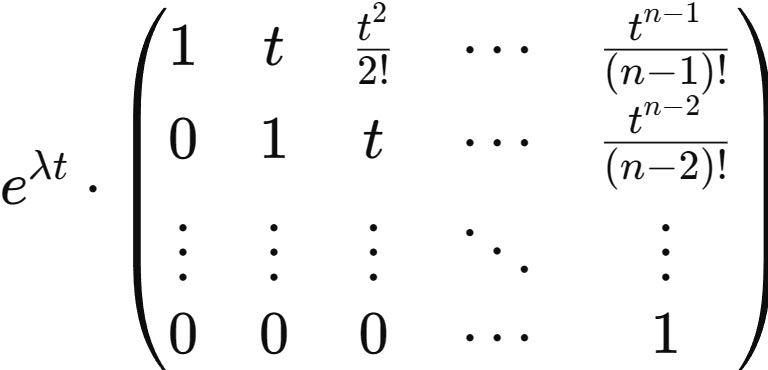
\includegraphics[width=1.0\textwidth]{pic1.jpg}
\end{minipage}

\textbf{Exponential of a matrix}: Given $P=A$ constant matrix, then \ $e^{Ax}:=\sum_{n=0}^{\infty}\frac{(Ax)^n}{n!}=\mathbb{I}+Ax+\frac{1}{2!}A^2x^2+\cdots,=\lim_{n\to\infty}(\mathbb{I}+\frac{Ax}{n})^n$

$\cdot$ Let $A,B$ be matrix. Then \textbf{1}. $e^{A+B}=e^{A}e^{B}$ if $AB=BA$ \ \ \ \textbf{2}. $e^{A\cdot0}=\mathbb{I}$ \ \ \ \textbf{3}. $\frac{d(e^{Ax})}{dx}=Ae^{Ax}$ {\scriptsize 和上面solve $\mathbf{y}'=A\mathbf{y}$相关}

\textbf{Solve $\mathbf{y}'=A\mathbf{y}$ (way 4)}: {\tiny 接着1.}{\scriptsize (For each $\xi_\lambda$, under $\lambda$)} {\small $\mathbf{y}^{(1)}=e^{\lambda x}\xi_\lambda$ \ \ $\mathbf{y}^{(2)}=e^{\lambda x}(x\xi_\lambda+\eta_1)$ \ \ $\mathbf{y}^{(3)}=e^{\lambda x}(\frac{x^2}{2!}\xi_\lambda+x\eta_2+\eta_1)$, ... ,$y^{(n)}=e^{\lambda x}[\frac{x^{n-1}}{(n-1)!}\xi_\lambda+\sum_{i=0}^{n-2}\frac{x^{i}}{(i)!}\eta_{i+1}]$}

{\scriptsize or 接着3} Let $T=[\lambda_1,...,\lambda_i,\eta^{(i)}_1,...,\lambda_j,\eta^{(j)}_1,...]$. \ $J=T^{-1}AT$ (Jordan form) \ \ \ $\mathbf{y}'=T\mathbf{z}$ $\Rightarrow [\mathbf{y}'=A\mathbf{y}\Leftrightarrow\mathbf{z}'=J\mathbf{z}]$,easy to solve $\mathbf{z}'=J\mathbf{z}$. {\tiny ps: $e^{J_i t}$ 见上图}


\subsection{Solve $\mathbf{y}'=A\mathbf{y}+\mathbf{g}$}

\vspace{-0.25cm}
{\tiny * 此节默认都是 Given constant matrix $A$, $\mathbf{y}'=A\mathbf{y}+\mathbf{g}$ (\star\star) \ \ \ \textbf{对于 Variation of Parameters 方法, A可以为P(任意矩阵函数)} \ \ \ \ \ \ \ \ \ \ \ \ \ \ \ \ \ Calculate $\lambda_j,\xi_j$ of $A\xi=\lambda\xi$ \ \ \ \ \ \ Let $T=[\xi_1,...,\xi_n],D=diag(\lambda_1,...,\lambda_n)$ (If it's possible, or to Jordan form)}

\vspace{-0.25cm}
{\tiny * 此节中，给出的都是如果是关于 initial value 的解时: 要 general solution 时, $\mathbf{y}_g$部分有关initial value的部分可以用$\mathbf{c}$代替, $\mathbf{y}_g$部分有关initial value 部分时,可以任意取值}
\vspace{-0.15cm}

\textbf{Theorem}: General solution of (\star\star) is of the form: $\mathbf{y}=\sum_ic_i\mathbf{y}^{(i)}+\mathbf{y}_{p}$, \ \ where $\mathbf{y}^{(i)}$ is solution of (\star). \ \ \ \ \ \ \ \ \ \ \ \ \ \ \ \ \ \ \ \ \ \ \ \ \ {\tiny $\Downarrow$ 通常会让特解中积分后的常数c=0}

\textbf{Variation of Parameters}: $\mathbf{y}=\mathbf{y}_g+\mathbf{y}_p$; \ \ \ $\mathbf{y}_g=\Psi(x)\Psi^{-1}(x_0)\mathbf{y}(x_0)$; \ \ \ $\mathbf{y}_p=\Psi(x)\mathbf{u}(x),\mathbf{u}(x)=\int^x_{x_0}\Psi^{-1}(s)\mathbf{g}(s)ds$. \ \ {\scriptsize 经常$\Psi(x)\mathbf{u}'=\mathbf{g}$来找$\mathbf{u}$}

\textbf{Diagonalisation {\footnotesize (matrix methods)}}: $^1$Let $\mathbf{y}=T\mathbf{z}$ \ \ \ $^2(\star\star)\Rightarrow \mathbf{z}'=D\mathbf{z}+T^{-1}\mathbf{g}=D\mathbf{z}+\mathbf{h}$ \ \ \ $^3$ {\tiny 直接计算;} $z_i=c_ie^{r_ix}+\underline{e^{r_ix}\int^x_{x_0}e^{-r_is}h_i(s)ds}_{\mathbf{y}_p}$

\vspace{-6pt}
{\scriptsize or,由上面 Way 4 得到 $T, J$. } $^1$Let $\mathbf{y}=T\mathbf{z}$ \ \ \ $^2(\star\star)\Rightarrow \mathbf{z}'=J\mathbf{z}+T^{-1}\mathbf{g}=J\mathbf{y}+\mathbf{h}$ \ \ \ $^3$ {\tiny 直接计算;可能会遇到$y'+p(x)y=q(x)$的形式}

\textbf{Undetermined Coefficients}: {\footnotesize when $\mathbf{g}(x)$ is \underline{polynomials}, or \underline{real/complex exponential}.} \ \ \ Let {\footnotesize $P_n(x)=\sum^n_{i=0}\mathbf{p}_ix^i,A_n(x)=\sum^n_{i=0}\mathbf{a}_ix^i$}

$^1${\scriptsize 构造$\mathbf{y}_p$与$\mathbf{g}$ 结构相匹配.(e.g. If $\mathbf{g}=P_n(x)\Rightarrow \mathbf{y}_p=A_n(x)$; If $\mathbf{g}=\mathbf{c}e^{kx}\Rightarrow \mathbf{y}_p=\mathbf{a}e^{kx}$)} \ $^2$ {\scriptsize 特殊: If $\mathbf{g}=\mathbf{c}e^{\lambda x}$,$\lambda$ is eigenvalue with $AM=n\Rightarrow \mathbf{y}_p=e^{\lambda x}\sum_{i=0}^{n}\mathbf{a}_ix^i$} \ $^3${\scriptsize 带入原方程得未知系数}


\subsection{Geometrical Interpretation \& Linear Approximation}

\vspace{-0.25cm}
{\tiny * 此节中，Consider nonlinear autonomous system: $x'=F(x,y),y'=G(x,y)$ (\ast\ast)}
\vspace{-0.15cm}

\textbf{Phase Plane}: {\small $O_{xy}$ referred as phase plane. \ \ \ \textbf{Trajectories}: Sol of ODE. $\mathbf{x}(t)=(x(t),y(t))^T$ {\tiny direction $(dx/dt,dy/dt)$} \ \ \ \textbf{Phases Portrait}:{\scriptsize 一组有代表性的轨迹}}

\textbf{Critical Point (Equilibrium Point)}: $\mathbf{x}_0=(x_0,y_0)$ is critical point iff $[x'=F(\mathbf{x}_0)=0,y'=G(\mathbf{x}_0)=0]$ {\scriptsize or} $[\mathbf{x}'=\mathbf{0}]$ {\tiny (critical point外变化简单)}

\textbf{Stable}: Critical Point $\mathbf{x}_0$ is stable \ \ iff \ \ $\forall\varepsilon>0,\exists\delta>0$ s.t. $\forall$ sols $\mathbf{x}(t)$ with $||\mathbf{x}(0)-\mathbf{x}_0||<\delta$, then $||\mathbf{x}(t)-\mathbf{x}_0||<\varepsilon$,$\forall t\geq0$

$\cdot$ {\footnotesize 直观理解:一开始离 critical point 很近,那么随着时间推移也会保持在 critical point 附近. \ \ \ ps:attrcting 是会趋近于 critical point.}

\textbf{Attracting}: Critical point $\mathbf{x}_0$ is attracting \ \ iff \ \ $\exists\delta>0$ s.t. $\forall$ sols $\mathbf{x}(t)$ with $||\mathbf{x}(0)-\mathbf{x}_0||<\delta$ satisfies: $\lim_{t\to\infty}\mathbf{x}(t)=\mathbf{x}_0$

\textbf{Asymptotically Stable}: Critical point $\mathbf{x}_0$ is asy.stab \ \ iff \ \ $^1$ Stable, $^2$ Attracting.

\textbf{Theorem}: If $\mathbf{x}_\ast(t)=(x_\ast,y_\ast)$ s.t. $F(\mathbf{x}_\ast),G(\mathbf{x}_\ast)\ne0$. \ \ $\Rightarrow$ \ \ $\exists H$ s.t. $H(x,y)=(\tilde{x},\tilde{y}),\tilde{x}'=1,\tilde{y}'=0$ {\tiny H is a smooth change of variable function in neighbourhood of $\mathbf{x}_\ast$}

\textbf{Non-Linear $\to$ Linear}: For system (\ast\ast), assume $\mathbf{x}_0=(x_0,y_0)$ is critical point. \ $\Rightarrow$ \ $\mathbf{u}=\mathbf{x}-\mathbf{x}_0$, then $\mathbf{u}'\approx A\mathbf{u}${\tiny \ Linear;} {\tiny $A=\begin{pmatrix}\partial_xF(\mathbf{x}_0) & \partial_yF(\mathbf{x}_0) \\ \partial_xG(\mathbf{x}_0) & \partial_yG(\mathbf{x}_0) \\ \end{pmatrix}$} {\tiny Jacobian}


\subsection{Classification of Critical Points}

\vspace{-0.25cm}
{\tiny * 此节中，Consider linear system: $\mathbf{x}'=A\mathbf{x}$. \ \ \ \ \ \ Critical Point(s): when $\mathbf{x}'=A\mathbf{x}=\mathbf{0}$}
\vspace{-0.15cm}

\textbf{Classification of Critical Points at $(x_0,y_0)$ (Linear)}: Let $r_1,r_2$ be sol of $det(A-\lambda I)=0$. \ \ \ \ \ \ $\cdot$ $\mathbb{C}:r=\lambda\pm i\mu(\mu>0)$

$\cdot$ If $A$ constant, write sol: $\mathbf{x}=c_1e^{r_1t}\xi_1+c_2e^{r_2t}\xi_2$ \ \ \ \ \ \ $\cdot GM=1$: $\mathbf{x}=c_1e^{rt}\xi+c_2e^{rt}(t\xi+\eta)$ \ \ \ \ \ \ $\cdot$ AL: Almost Linear Systems.

\vspace{-8pt}
\begin{longtable}{|c|c|c|l|l|}
    \hline
    {\tiny $\mathbb{R} / \mathbb{C}$} & {\scriptsize Condition || Stability} & Type || Name & Phase Plane Description & Other \\
    \hline
    \multirow{7}{*}{$\mathbb{R}$} & {\scriptsize $r_1<r_2<0$ || asy.stab} & {\small N || NSk} & {\tiny 向原点,$\xi_2$直线,$\xi_1$曲线,and $\xi_1$周围$y=\pm x^3$} & {\scriptsize $c_2\ne0,t\to\infty$:$\xi_2$主导方向; \ $c_2=0,t\to\infty$:$\xi_1$主导方向} \\
    \cline{2-5}
    & {\scriptsize $r_1>r_2>0$ || unstable} & {\small N || NSo} & {\tiny 原点向外,$\xi_2$直线,$\xi_1$曲线,and $\xi_1$周围$y=\pm x^3$} & {\scriptsize $c_1\ne0,t\to\infty$:$\xi_1$主导方向; \ $c_1=0,t\to\infty$:$\xi_2$主导方向} \\
    \cline{2-5}
    & {\scriptsize $r_1>0>r_2$ || unstable} & SP || SP & \makecell{\scriptsize $t\to\infty$,$\xi_1$从原点向外,$\xi_2$从外向原点 \\ \scriptsize and: 像$y=\pm\frac{1}{x}$,同进同出} & \makecell{\scriptsize $t\to\pm\infty:|\mathbf{x}|\to\infty$; \ \ \ \ \ $t\to\infty:c_1,c_2\ne0,|\mathbf{x}|\to\infty$,$\xi_1$主导; \ \ \ \ \ \ \ \ \ \ \ \ \ \ \ \ \ \\ \scriptsize $t\to\infty:c_2=0,|\mathbf{x}|\to\infty$,$\xi_1$主导; \ \ \ \ $t\to\infty:c_1=0,|\mathbf{x}|\to0$,$\xi_2$主导} \\
    \cline{2-5}
    & {\scriptsize $r_1=r_2<0$, {\tiny GM=2} || {\tiny asy.stab}} & {\small PN || {\scriptsize PN or Stable Star}} & {\scriptsize \underline{直线}向原点} & {\scriptsize 直线, $u_1/u_2$ is $t$ independent} \\
    \cline{2-5}
    & {\scriptsize $r_1=r_2>0$, {\tiny GM=2} || {\tiny unstable}} & {\small PN || {\scriptsize PN or Unstable Star}} & {\scriptsize \underline{直线}从原点向外} & {\scriptsize 直线, $u_1/u_2$ is $t$ independent} \\
    \cline{2-5}
    & {\scriptsize $r_1=r_2<0$, {\tiny GM=1} || {\tiny asy.stab}} & {\small IN {\tiny(AL:Type: SpP)} || {\scriptsize IN {\tiny (Stable)}}} & {\scriptsize S曲线,向原点} & {\scriptsize $t\to\infty,|\mathbf{x}|\to0,\xi$主导 \ \ \ \ \ \ ps:旋转方向大体和$\eta+c_2\xi$方向相同} \\
    \cline{2-5}
    & {\scriptsize $r_1=r_2>0$, {\tiny GM=1} || {\tiny unstable}} & {\small IN {\tiny(AL:Type: SpP)} || {\scriptsize IN {\tiny (Unstable)}}} & {\scriptsize S曲线,从原点向外} & {\scriptsize $t\to\infty,|\mathbf{x}|\to\infty,\xi$主导 \ \ \ \ \ \ ps:旋转方向大体和$\eta+c_2\xi$方向相同} \\
    \hline
    \multirow{3}{*}{$\mathbb{C}$} & {\scriptsize $\lambda\ne0,\lambda>0$ || unstable} & {\small SpP || Unstable Focus} & {\scriptsize 向外椭圆(elliptical)螺旋} & {\scriptsize $t\to\infty,|\mathbf{x}|\to\infty$ \ \ \ {\tiny ps:考虑$A=(a,b;c,d)$,如果bc>0,顺时针，如果bc<0,逆时针}} \\
    \cline{2-5}
    & {\scriptsize $\lambda\ne0,\lambda<0$ || asy.stab} & {\small SpP || Stable Focus} & {\scriptsize 向内椭圆(elliptical)螺旋} & {\scriptsize $t\to\infty,|\mathbf{x}|\to0$ \ \ \ {\tiny ps:考虑$A=(a,b;c,d)$,如果bc>0,顺时针，如果bc<0,逆时针}} \\
    \cline{2-5}
    & {\scriptsize $\lambda=0$ || stable {\tiny (AL:Indeterminate)}} & {\small C {\scriptsize (AL:C or SpP)} || C} & {\scriptsize 椭圆(elliptical) and 半长轴$\xi$实部方向} & {\scriptsize Bounded trajectory \ \ \ or \ \ \ $\exists$ Periodic Trajectories} \\
    \hline
    \multicolumn{5}{|l|}{\scriptsize ps: N = Node | PN = Proper Node | IN = Improper / Degenerate Node | SP = Saddle Point | SpP = spiral (focus) point | C = Center | NSk = Nodal Sink | NSo = Nodal Source} \\
    \hline
    \multicolumn{5}{|l|}{\scriptsize For Almost Linear systems (见2.5): $\mathbf{u}'=A\mathbf{u}+\underline{\eta}$, 如果 linear Approximation (去掉$\underline{\eta}$),按照 Linear 考虑. \ \ \ \ \ \ 如果不去$\underline{\eta}$,按照去掉的算$r_1,r_2$, Type 按照 正常 / (AL) 的来.{\tiny(图像会到$(0,0)$)}} \\
    \hline
\end{longtable}
\vspace{-0.4cm}

\textbf{Some Defs}: {\scriptsize $Separatrix$:将不同区域分开的轨迹; \ \ \ $Basin \ of \ attraction$: 所有趋近critical point的轨迹.} \ \ \ {\tiny ps: In any nonlinear ODEs, it's important to determine the \textit{basin of attraction}.}


\subsection{Non-Linear Methods}

\vspace{-0.25cm}
{\tiny * 此节中，Consider two-dimensional autonomous system: $x'=F(x,y)$, $y'=G(x,y)$ and $\mathbf{x}=(x,y)^T$ (\#) \ \ \ \ \ \ Lyapunov's: 不需要知道微分方程的确切解critical value. \ \ \ \ \ \ Poincaré-Bendixson:寻找limit cycle}
\vspace{-0.15cm}

\textbf{Positive (Negative) [semi-]definite}: Function $E:D\subset\mathbb{R}^2\to\mathbb{R}$ is positive (negative) [semi-]definite iff: \ \ {\tiny ps: positive [semi-]definite 正(半)定}

\ \ \ \ \ \ \ \ \ \ \ \ \ \ \ \ \ \ \ \ \ \ \ \ \ \ \ \ \ \ \ \ \ \ \ \ \ \ \ \ \ \ \ \ \ \ \ \ \ \ \ \ \ \ \ \ \ \ \ \ \ \ \ \ \ \ \ \ \ \ \ \ \ $^1E(\mathbf{x}_0)=0$, $^2\forall\mathbf{x}\in D,\textbf{x}\ne\mathbf{x}_0,E(x,y)>0$ \ {\scriptsize or $(E(x,y)<0)$ \ or \ $[E(x,y)\geq0]$} \ \ {\tiny ps: Neighbourhood 领域}

\textbf{Isolated Critical Point}: Critical Point $\mathbf{x}_0$ \textit{isolated} iff $\exists$ Neighbourhood containing no other critical points. \ \ \ \ \ \ \ \ \ \ \ {\footnotesize $\downarrow \Rightarrow E:$Lyapunov function}

\textbf{Lyapunov Stability Theorem}: {\scriptsize $^1$(\#); $^2$ICP $\mathbf{x}_0\in D$; $^3\exists$ 正定 且 连续 $ E:D\subset\mathbb{R}^2\to\mathbb{R},E(\mathbf{x}_0)=0$; || $^4\frac{dE}{dt}=\nabla E\cdot\mathbf{x}'=\partial_x E\cdot F+\partial_y E\cdot G$ 负(半)定 on $D\setminus\mathbf{x}_0(D)$} $\Rightarrow$ {\footnotesize $\mathbf{x_0}$ asp.(stab)}

$\cdot$ \textbf{Look for function $E$}: {\footnotesize Way 1: May be energy, but not always. \ \ \ \ \ \ Way 2: \textit{e.g.} $E=ax^{2n}+by^{2m}$,$E=a(x+y)^{2n}+by^{2m}$ \ ps: $\frac{dE}{dt}=\nabla E\cdot\mathbf{x}'$}

\textbf{Lyapunov Instability Theorem}: {\footnotesize $^1$(\#); $^2$ICP $\mathbf{x}_0\in D$; $^3\exists E:D\subset\mathbb{R}^2\to\mathbb{R},\partial_i E$ 连续,$E(\mathbf{x}_0)=0$; $^4\forall${\tiny 领域}$\mathbf{x}_0,\exists\mathbf{x}_1 \ E(\mathbf{x}_1)>0$; || $^5\frac{dE}{dt}$ 正定 on $D$ $\Rightarrow$ $\mathbf{x_0}$ unstable}

\textbf{Periodic Solution}: {\scriptsize Soln $\mathbf{x}$ has: $\mathbf{x}(t+T)=\mathbf{x}(t),\forall x$}.  || {\scriptsize 闭合曲线 $\Leftrightarrow$ Periodic sol} || {\scriptsize Periodic Solution + 附近有吸引或排斥 $\Rightarrow$ Limit Cycle} || {\scriptsize when $\dot{r}=0,\dot{\theta}=const.$ Periodic sol}

\textbf{Limit cycle}: {\scriptsize Limit cycle $\Rightarrow$ Periodic Solution} || Def $t\to\pm\infty,\exists$ non-closed trajectory asymptotes to it. {\scriptsize (inside or outside)} \ \ \ \ \ \ {\scriptsize ps: It's Orbital Stability}
\begin{enumerate}[itemsep=-2pt, topsep=-2pt]
    \item Limit cycle is: $^1$asy.stab: $\forall$ trajectories asy. it; \ \ \ $^2$semistable: $\exists$ trajectories {\footnotesize 单方向 进/出}; \ \ \ $^3$unstable: $\forall$ trajectories away from it.
    \item \textbf{Theorem (If $\exists$ limit cycle / closed)}: {\footnotesize $^1F,G${\scriptsize 一阶偏导连续} in simply connected $D$; $^2\exists$ {\scriptsize 极限环/封闭环} (\star) in $D$. \ $\Rightarrow$ \ $^1\exists$ CP in (\star); $^2$If $\exists!$ CP in (\star), it's not SP}.
    \item \textbf{Theorem (No limit cycle / closed)}: {\footnotesize $^1F,G$一阶偏导连续 in simply connected $D$; $^2\partial_xF+\partial_yG$符号不变 on D \ $\Rightarrow$ \ No closed trajectory in D.}
    \\ {\footnotesize 2的推论: $^1$If simple connected $D$ no CP \ $\Rightarrow$ \ No closed trajectory in D. \ \ \ \ \ \ $^2$If simple connected D has unique CP \ $\Rightarrow$ \ No closed trajectory in D}
\end{enumerate}

\textbf{Poincaré-Bendixson Theorem}: {\footnotesize $^1F,G$一阶偏导连续 in $D$; \ \ $^2\exists D_1\subset D$ bounded; \ \ $^3R=D_1\cup\partial D_1$ has NO CP; \ || \ $^4$ $\exists$ soln $\mathbf{x}\in R$, $\forall t\geq t_0$ \ $\Rightarrow$}

\ \ \ \ \ \ \ \ \ \ \ \ \ \ \ \ \ \ \ \ \ \ \ \ \ \ \ \ \ \ \ \ \ \ \ \ \ \ \ \ \ \ \ \ \ \ \ \ \ \ \ \ \ \ \ \ \ \ \ \ \ \ \ \ \ \ {\footnotesize $\Rightarrow$ $^1\exists$ closed trajectory. \ \ \ \ \ \ $^2$ Either \textit{$\mathbf{x}$ sprial towards a Periodic trajectory.} \ or \ \textit{$\mathbf{x}$ periodic}} \ \ \ \ \ \ {\footnotesize $^3R$ is not simply connected}

$\cdot$ \textbf{Find Trapping Region}: {\scriptsize \textbf{trapping region}: 符合上面定理2-4除CP的region. \ \ \ \ Method: Consider \textit{polar coordinate}, 计算$r^2=x^2+y^2$ 对 $t$的求导, 寻找$r\dot{r}\geq0$ or $r\dot{r}\leq0$}


\section{Fourier Series}

\vspace{-0.25cm}
\hspace{20pt}{\tiny * BVPs 可能没有解/一个解/无数解; IVP 只会有一个解}
\vspace{-0.15cm}

\subsection{Function Space, Eigenfunctions, Periodic Function and Orthogonal Function}

\textbf{Differential Operators}: Any linear combination of $n$-th derivatives defines a linear map or linear operator. \ \ \ \ \ \ {\tiny e.g. $p(x)\frac{d}{dx}+\frac{d^2}{dx^2}:y\mapsto p(x)\frac{dy}{dx}+\frac{d^2y}{dx^2}$}

\textbf{Eigenvalues \& Eigenfunctions}: If $D$ is a \textit{differential operator} \ $\Rightarrow$ \ If $Df=\lambda f$, then $\lambda$ is \textbf{Eigenvalue} and $f$ is \textbf{Eigenfunctions}

\textbf{Periodic Functions}: Function $f(x)$ is Periodic iff $f(x+T)=f(x),\forall x$. \ \ \ \textbf{Period}: T. \ \ \ \textbf{Fundamental Period}: The smallest possible T.

$\cdot$ Property: If $f,g$ has same period $T$. \ $\Rightarrow$ \ $af(x)+bg(x)$ also has period $T$. \ \ \ || \ \ \ For $sin(\omega x),cos(\omega x)$: $T=2\pi/\omega$

\textbf{Inner Product of functions}: func $f,g$ in the interval $[a,b]$ \ $\Rightarrow$ \ Inner Product: $(f,g) =\int^b_af(x)g(x)dx$ || \textbf{Orthogonal}: $(f,g)=0$

$\cdot$ Important Situation: Set $\{sin(\frac{n\pi x}{L}),cos(\frac{m\pi x}{L})\}$ Orthogonal each pair (\textbf{Mutually orthogonal}) in the interval $[-L,L]$.

\textbf{Kronecker delta}: $\delta_{mn}=\{0,m\ne n; \ 1,m=n.$


\subsection{Fourier Series}

\textbf{Fourier Series}: Periodic function with $T=L$ \ , \ $f(x)=\frac{a_0}{2}+\sum_{n=1}^{\infty}\left(a_ncos(\frac{n\pi x}{L})+b_nsin(\frac{n\pi x}{L})\right)$ (*) \ \ \ {\tiny where $a_0,a_n,b_n$ are determined by \textit{Euler-Fourier Formulas}.}

\textbf{Euler-Fourier Formulas}: Suppose (*) converges in the interval $[-L,L]$. Then:

\hspace{116pt}$a_n=\frac{1}{L}\int^L_{-L}f(x)cos(\frac{n\pi x}{L})dx$ \ \ \ \ \ \ \ \ \ \ \ \ $b_n=\frac{1}{L}\int^L_{-L}f(x)sin(\frac{n\pi x}{L})dx$ \ \ \ \ \ \ \ \ \ \ \ \ $a_0=\frac{1}{L}\int^L_{-L}f(x)dx$


\section{Appendix}

\textbf{Trigonometric func}: {\footnotesize s+s=sc,s-s=cs,c+c=cc,c-c=-ss || e.g. $sinA+sinB=2sin(\frac{A+B}{2})cos(\frac{A+B}{2})$ \ \ \ $sinAsinB=-\frac{1}{2}[cos(A+B)-cos(A-B)]$}

\textbf{hyperbolic func}: {\footnotesize $sinh(x)=\frac{e^x-e^{-x}}{2}$ \ \ \ $cosh(x)=\frac{e^x+e^{-x}}{2}$ \ \ \ $cosh^2(x)-sinh^2(x)=1$ \ \ \ $[sinh(x)]'=cosh(x)$ \ \ \ $[cosh(x)]'=sinh(x)$}

\textbf{Common Int}: {\footnotesize $\int tan(x)dx=-ln|cos(x)|$; \ \ $\int cot(x)dx=ln|sin(x)|$; \ \ $\int sec(x)dx = ln|sec(x)+tan(x)|$; \ \ $\int csc(x)dx = ln|csc(x)-cot(x)| = ln|tan(\frac{x}{2})|$}

\textbf{Common Der}: {\footnotesize $[tan(x)]'=sec^2(x)$; \ \ $[cot(x)]'=-csc^2(x)$; \ \ $[sec(x)]'=sec(x)tan(x)$; \ \ $[csc(x)]'=-csc(x)cot(x)$; \ \ $[arctan(x)]'=\frac{1}{1+x^2}$.}

$\cdot$  {\footnotesize $1+tan^2(x)=sec^2(x)$; \ \ $1-csc^2(x)=cot^2(x)$; \ \ $csc^2(x)-cot^2(x)=1$. \ \ \ \ \ \ \ \ \ \ \ \ \ \ \ \ \ \ \ \ \ \ \ \ \ \ \ \ \ \ \ \ \ \ \ \ \ \ \ \ \ \ \ \ \ \ \ $[arcsin(x)]'=\frac{1}{\sqrt{1-x^2}}$; \ \ $[arccos(x)]'=-\frac{1}{\sqrt{1-x^2}}$}

\textbf{Polar Coordinate}: $x=rcos(\theta)$,$y=rsin(\theta)$ \ \ \ \ \ \ we have: $r\dot{r}=x\dot{x}+y\dot{y}$ \ , \ $y\dot{x}-x\dot{y}=-r^2\dot{\theta}$

\end{document}